% Copyright 2020 by Robert Hildebrand
%This work is licensed under a
%Creative Commons Attribution-ShareAlike 4.0 International License (CC BY-SA 4.0)
%See http://creativecommons.org/licenses/by-sa/4.0/

%\documentclass[../open-optimization/open-optimization.tex]{subfiles}
%
%\begin{document}

\chapter{Exponential Size Formulations}
\label{sec:exponential-IP-forumulations}
\todoChapter{ 60\% complete. Goal 80\% completion date: August 20\\
Notes: }
\begin{outcome}
We will learn two fundamental tools to be used in optimization.  The desired outcomes are:
\begin{itemize}
\item Understand column generation and how generating solutions templates/patterns can be extremly powerful.
\item Understand how cutting plane schemes can be applied when there are exponentially many constraints.
\end{itemize}

\end{outcome}

Although typically models need to be a reasonable size in order for us to code them and send them to a solver, there are some ways that we can allow having models of exponential size.  The first example here is the cutting stock problem, where we will model with exponentially many variables.  The second example is the traveling salesman problem, where we will model with exponentially many constraints.  We will also look at some other models for the traveling salesman problem.  
\section{Cutting Stock}
This is a classic problem that works excellent for a technique called \emph{column generation}.
We will discuss two versions of the model and then show how we can use column generation to solve the second version more efficiently.  First, let's describe the problem.

\begin{general}{Cutting Stock}{}
You run a company that sells of pipes of different lengths.  These lengths are $L_1, \dots, L_k$.  To produce these pipes, you have one machine that produces pipes of length $L$, and then cuts them into a collection of shorter pipes as needed.  

\begin{center}
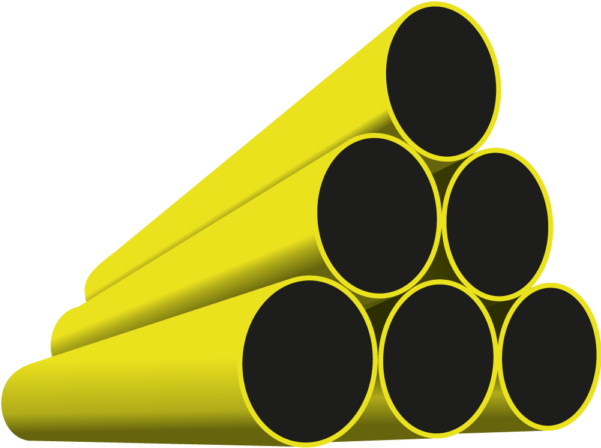
\includegraphics[scale = 0.2]{pipes}\footnote{
\url{https://www.pinclipart.com/pindetail/TihJbb_stacks-of-pipe-steel-casing-pipe-clipart/}}
\end{center}

You have an order come in for $d_i$ pipes of length $i$ for $i=1, \dots, k$.  How can you fill the order while cutting up the fewest number of pipes?
\end{general}
\begin{example}{Cutting stock with pipes}{cuttingStockPipe}
A plumber stocks standard lengths of pipe, all of length 19 m. An order arrives for:
\begin{itemize}
\item  12 lengths of 4m
\item 15 lengths of 5m
\item 22 lengths of 6m
\end{itemize}
How should these lengths be cut from standard stock pipes so as to minimize
the number of standard pipes used?
\end{example}
\begin{center}
%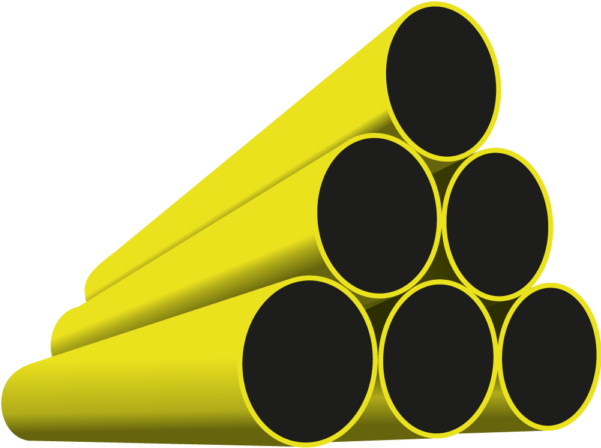
\includegraphics[scale = 0.1]{pipes}
%https://www.freeimages.com/search/sawing-pipe
\end{center}

An initial model for this problem could be constructed as follows:  
\begin{itemize}
\item Let $N$ be an upper bound on the number of pipes that we may need.
\item Let $z_j = 1$ if we use pipe $i$ and $z_j = 0$ if we do not use pipe $j$, for $j=1, \dots, N$.
\item Let $x_{ij}$ be the number of cuts of length $L_i$ in pipe $j$ that we use.
\end{itemize}
Then we have the following model
\begin{equation}
\begin{split}
\min\ \  & \sum_{j=1}^N z_j\\
\st \ \  & \sum_{i=1}^k  L_i x_{ij} \leq Lz_j \ \text{ for } j=1,\dots, N\\
& \sum_{j=1}^N x_{ij} \geq d_i \ \text{ for } i=1, \dots, k\\
& z_j \in \{0,1\} \text{ for } j=1, \dots, N\\
& x_{ij} \in \Z_+ \text{ for } i=1, \dots, k,\, j=1, \dots, N
\end{split}
\end{equation}
\begin{exercise}{Show Bound}{}
In the example above, show that we can choose $N=16$.
\end{exercise}
\begin{examplewithcode}{}{https://github.com/open-optimization/open-optimization-or-examples/blob/master/integer-programming/cutting-stock.ipynb}{}{}

For our example above, using $N=16$, we have
\begin{equation}
\begin{split}
\min\ \  & \sum_{j=1}^{16} z_j\\
\st \ \  &  4 x_{1j} + 5 x_{2j} + 6 x_{3j} \leq 19 z_j\\
& \sum_{j=1}^{16} x_{1j} \geq 12\\
& \sum_{j=1}^{16} x_{2j} \geq 15\\
& \sum_{j=1}^{16} x_{3j} \geq 22\\
& z_j \in \{0,1\} \text{ for } j=1, \dots, 16\\
& x_{ij} \in \Z_+ \text{ for } i=1, \dots, 3,\, j=1, \dots, 16
\end{split}
\end{equation}
Additionally, we could break the symmetry in the problem.  That is, suppose the solution uses 10 of the 16 pipes.  The current formulation does not restrict which 10 pipes are used.  Thus, there are many possible solutions.  To reduce this complexity, we can state that we only use the first 10 pipes.  We can write a constraint that says \emph{if we don't use pipe $j$, then we also will not use any subsequent pipes}.  Hence, by not using pipe 11, we enforce that pipes $11, 12, 13, 14,15,16$ are not used.  This can be done by adding the constraints
\begin{equation}
z_1 \geq z_2 \geq z_3 \geq \dots \geq z_N.
\end{equation}

\end{examplewithcode}

Unfortunately, this formulation is slow and does not scale well with demand.  In particular, the number of variables is $N + kN$ and the number of constraints is $N$ (plus integrality and non-negativity constraints on the variables).  
The solution times for this model are summarized in the following table:
\begin{table}
\begin{tabular}{ccccccccccccc}
\hline
demand muliplier & 1& 10& 100& 500& 1000& 10000& 100000& 200000& 400000\\
\hline
board model time (s) & 0.0517& 0.6256& 24.32& 600\\
pattern model time (s) & 0.0269&
 0.0251&
 0.0289&
 0.0258&
 0.0236&
 0.0202&
 0.022&
 0.0186&
 0.0204\\
 \hline
 \end{tabular}
 \caption{Table comparing computaional time in the two models.  We stopped computations at 600 seconds.   Notice that the pattern model does not care how large the demand is - it still solves in the same amount of time!  The demand multiplier $k$ here means that we multiply $k$ times the demand vector used in the example.  This grows the number of variables in the Board based model, but doesn't change much in the pattern based model.}
\end{table}



\subsection{Pattern formulation}
We could instead list all patterns that are possible to cut each pipe.   A pattern is an vector $a \in \Z^k_+$ such that for each $i$, $a_i$ lengths of $L_i$ can be cut from a pipe of length $L$.  That is
\begin{equation}
\begin{split}
\sum_{i=1}^k &L_i a_i \leq L\\
a_i &\in \Z_+ \ \text{for all } i=1, \dots, k
\end{split}
\end{equation}
In our running example, we have 
\begin{equation}
\begin{split}
4 &a_1 + 5 a_2 + 6 a_3 \leq 19\\
&a_i \in \Z_+ \ \text{for all } i=1, \dots, 3
\end{split}
\end{equation}


For visualization purposes, consider the patterns where $a_3 = 0$.  That is, only patterns with cuts of length 4m or 5m.  All patterns of this type are represented by an integer point in the polytope 
\begin{equation}
P = \{(a_1,a_2) : 4a_1 + 5 a_2 \leq 19, a_1\geq 0, a_2 \geq 0\}
\end{equation}
which we can see here:
\begin{center}
\includegraphicstatic[scale = 0.4]{knapsack_fig.pdf}
\end{center}
where $P$ is the blue triangle and each integer point represents a pattern.  Feasible patterns lie inside the polytope $P$.  Note that we only need patterns that are maximal with respect to number of each type we cut.  Pictorially, we only need the patterns that are integer points represented as yellow dots in the picture below.
\begin{center}
\includegraphicstatic[scale = 0.4]{knapsack_fig_maximal.pdf}
\end{center}
For example, the pattern $[3,0,0]$ is not needed (only cut 3 of length 4m) since we could also use the patten $[4,0,0]$ (cut 4 of  length 4m) or we could even use the pattern $[3,1,0]$  (cut 3 of length 4m and 1 of length 5m).

\begin{example}{Pattern Formulation}{}
Let's list all the possible patterns for the cutting stock problem:

\begin{center}
\begin{tabular}{l|c|c|c|c|c|c|c|c|c|c}
& \multicolumn{7}{c}{Patterns}\\
\hline
Cuts of length 4m &0 &0 &1 &0 &2 &1 &2 &3 &4 & 1\\
 Cuts of length 5m   &    0 &1 &0 &2 &1 &2& 2& 1 &0&3 \\
 Cuts of length 6m   &    3& 2 &2 &1 &1 &0& 0& 0 &0 &0\\
 \hline
\end{tabular}
\end{center}

We can organize these patterns into a matrix.
\begin{equation}
A = 
\begin{pmatrix}
0 &0 &1 &0 &2 &1 &2 &3 &4 & 1\\
        0 &1 &0 &2 &1 &2& 2& 1 &0&3 \\
        3& 2 &2 &1 &1 &0& 0& 0 &0 &0
\end{pmatrix}
 \end{equation}
 
 Let $p$ be the number of patterns that we have.  We  create variables $x_1, \dots, x_p \in \Z_+$ that denote the number of times we use each pattern.

Now, we can recast the optimization problem as

\begin{align}
\min \ \ & \sum_{i=1}^p x_i \\
\text{such that} \ \ & Ax \geq \begin{bmatrix} 12 \\ 15 \\ 22\end{bmatrix}\\
& x \in \Z^p_+
\end{align}
 
\end{example}



\subsection{Column Generation}
Consider the linear program\eqref{LP:basis-solution}, but in this case we are instead minimizing.  


Thus we can write it as 
 \begin{equation}
 \label{LP:basis-solution2}
\begin{split}
\min \quad & (c_N  - c_B A_B^{-1} A_N) x_N + c_B A_B^{-1} b  \\
\st  \quad &x_B +  A_B^{-1} A_N x_N = A_B^{-1}b\\
& x \geq 0
\end{split}
\end{equation}
In our LP we have $c = \one$, that is, $c_i =1$ for all $i=1, \dots, k$.  Hence, we can write it as 
 \begin{equation}
 \label{LP:basis-solution3}
\begin{split}
\min \quad & (\one_N  - \one_B A_B^{-1} N) x_N + \one_B A_B^{-1} b  \\
\st  \quad &x_B +  A_B^{-1} A_N x_N = A_B^{-1}b\\
& x \geq 0
\end{split}
\end{equation}
Now, if there exists a non-basic variable that could enter the basis and improve the objective, then there is one with a reduced cost that is negative.  For a particular non-basic variable, the coefficient on it is
\begin{equation}
\left( 1 -  \one_B A_B^{-1} A_N^i\right) x_i
\end{equation}
where $A_N^i$ is the $i$-th column of the matrix $A_N$.  Thus, we want to look for a column $a$ of $A_N$ such that 
\begin{equation}
1 -  \one_B A_B^{-1} a < 0 \ \  \Rightarrow \ \   1 < \one_B A_B^{-1} a
\end{equation}
\begin{general}{Pricing Problem}{(knapsack problem!)}
Given a current basis $B$ of the \emph{master} linear program, there exists a new column to add to the basis that improves the LP objective if and only if the following problem has an objective value strictly larger than 1.
\begin{equation}
\begin{split}
\max\quad  &\one_B A_B^{-1} a\\
\st \quad & \sum_{i=1}^k L_i a_i \leq L\\
& a_i \in \Z_+ \text{ for } i=1, \dots, k
\end{split}
\end{equation}
\end{general}

\begin{example}{Pricing Problem}{(knapsack problem!)}
Let's make the initial choice of columns easy.  We will do this by selecting columns 

\begin{center}
\begin{tabular}{l|c|c|c|c|c|c|c|c|c|c}
& \multicolumn{3}{c}{Patterns}\\
\hline
Cuts of length 4m &4 & 0 & 0  \\ %&1 &0 &2 &1 &2 &3 &4 & 1\\
 Cuts of length 5m   & 0 &  3 &   0  \\%&1 &0 &2 &1 &2& 2& 1 &0&3 \\
 Cuts of length 6m   & 0 &  0 &  3 \\% & 2 &2 &1 &1 &0& 0& 0 &0 &0\\
 \hline
\end{tabular}
\end{center}

So our initial $A$ matrix is

\begin{equation}
A = 
\begin{pmatrix}
4 & 0 & 0 \\
          0 &  3 &   0 \\
         0 &  0 &  3 
\end{pmatrix}
 \end{equation}
 
 Notice that there are enough patterns in the initial $A$ matrix to produce feasible solution.  Let's also append an arbitrary column to the $A$ matrix as a potential new pattern.
 
 \begin{equation}
A = 
\begin{pmatrix}
4 & 0 & 0 & a_1 \\
          0 &  3 &   0  & a_2\\
        0 &  0 &  3  & a_3
\end{pmatrix}
 \end{equation}
 
 Now, let's solve the linear relaxation and compute the tabluea.
 
 
 
 
 

 


\begin{equation}
\begin{split}
\max\quad  & \tfrac14 a_1 + \tfrac 13 a_2 + \tfrac 13 a_3\\
\st \quad & 4 a_1 + 5 a_2 + 6 a_3 \leq 19\\
& a_i \in \Z_+ \text{ for } i=1, \dots, k
\end{split}
\end{equation}
We then add optimal solution to the master problem as a new column and repeat the procedure.
\end{example}

See \href{https://github.com/Gurobi/modeling-examples/blob/master/colgen-cutting_stock/colgen-cutting_stock.ipynb}{Gurobi - Cutting Stock Example} for an example of column generation implemented by the Gurobi team.

\subsection{Cutting Stock - Multiple widths}



Here are some solutions:
\begin{itemize}
\item  \url{https://github.com/fzsun/cutstock-gurobi}.
\item \url{http://www.dcc.fc.up.pt/~jpp/mpa/cutstock.py}
\end{itemize}


Here is an AIMMS description of the problem: 
\href{https://download.aimms.com/aimms/download/manuals/AIMMS3OM_CuttingStock.pdf}{AIMMS Cutting Stock}

% \beign{bmatrix} 1 \\ 1 \\ 1\end{bmatrix}


%\section{Spanning Trees}
%\label{sec:spanning-tree-models}
%\subsection{2.1 Cycle Prevention in MST}
%
%The Cycle Elimination Model presents a concise mathematical representation of the Minimum Spanning Tree (MST). In this formulation, we introduce a binary decision variable, \(x_a\), which denotes whether an arc \(a \in \mathcal{A}\) will be a part of the tree (\(x_a=1\)) or if it will be excluded (\(x_a=0\)). The model is articulated as:
%
%\textbf{Objective:}
%\[
%\text{Minimize} \ \sum_{a \in \mathcal{A}} l_a x_a
%\]
%
%\textbf{Constraints:}
%\begin{align*}
%&x_a \in\{0,1\} &\forall a \in \mathcal{A} \\
%&\sum_{a \in \mathcal{A}} x_a=n-1 \\
%&\sum_{a \in A(S)} x_a \leq |S|-1 &\forall S \subset \mathcal{N}, |S|>1
%\end{align*}
%
%\section{2.2 Node-Level MILP Formulation}
%
%Delving into a more sophisticated representation, we introduce a model inspired by the conceptual link between the branching structure of trees and the flow patterns observed in rivers. In this comparison, rivers, originating from multiple sources and culminating into a single end-point, mirror the branching nature of trees. Fundamental to both is the absence of cycles.
%
%To model this, we use the directed graph \(\mathcal{G}=(\mathcal{N}, \mathcal{D})\), as introduced in Section 2.3. Each node in \(\mathcal{N}\) is represented by binary decision variables \(z_d\), where \(d \in \mathcal{D}\). An arbitrary node, termed as \(\omega\), is designated as the 'sink'. Other nodes are treated as either water sources or intermediary junctions, ensuring that water flows from a higher-level node to a lower one.
%
%To capture the 'water level' at each node, decision variables \(V_i\) are defined for every \(i \in \mathcal{N}\). By default, the sink node has the minimum level (zero), while all other nodes possess a level greater than zero. The relationship between \(z_d\) variables and node levels is maintained using specific constraints. The formulation is presented below:
%
%\textbf{Objective:}
%\[
%\text{Minimize} \ \sum_{d \in \mathcal{D}} l_d z_d
%\]
%
%\textbf{Constraints:}
%\begin{align*}
%&\sum_{(i, j) \in \mathcal{D}} z_{(i, j)}=1 &\forall i \in \mathcal{N}-\{\omega\} \\
%&\sum_{(\omega, j) \in \mathcal{D}} z_{(\omega, j)}=0 \\
%&V_i \geq V_j+z_{(i, j)}-n\left(1-z_{(i, j)}\right) &\forall(i, j) \in \mathcal{D} \\
%&V_\omega=0 \\
%&z_d \in\{0,1\} &\forall d \in \mathcal{D}
%\end{align*}


%\includegraphics[scale = 0.6]{minimum-weight-spanning-tree}
%~\cite{MARTIN1991119}
%
%
%\includegraphics[scale = 0.5]{minimum-spanning-tree-ip-model}
%
%\includegraphics[scale = 0.5]{minimum-spanning-tree-model-comparison}
%
%\includegraphics[scale = 0.5]{minimum-spanning-tree-list-of-models}


\section{Traveling Salesman Problem}
\label{sec:tsp-models}
The Traveling Salesman Problem (TSP) stands as one of the most iconic and studied problems in the realm of operations research and combinatorial optimization. At its core, the TSP asks a seemingly simple question: Given a list of cities and the distances between each pair, what is the shortest possible route a salesman can take to visit each city exactly once and return to the original city? While the problem statement is straightforward, finding an optimal solution, especially for a large number of cities, is computationally challenging.

The significance of the TSP extends far beyond its basic premise. It has a myriad of practical applications, ranging from logistics and transportation planning to microchip manufacturing and DNA sequencing. The TSP has been a cornerstone in highlighting the challenges of optimization in real-world scenarios. Moreover, the quest to solve the TSP has led to the development of numerous groundbreaking algorithmic techniques and heuristics. These methods, inspired by the intricacies of the TSP, have found applications in a wide array of other optimization problems, further emphasizing the TSP's foundational role in the evolution of operations research.



\href{https://www.google.com/maps/dir/(38.2222341,+-85.75750389999999)/(39.0972041,+-84.52636389999999)/(38.0493956,+-84.4940986)/(37.1967465,+-80.4296817)/(37.2049884,+-79.9237747)/(37.5110489,+-77.40769019999999)/(35.2019605,+-80.81365720000001)/(36.1303318,+-86.78998039999999)/(38.2222341,+-85.75750389999999)/@36.8110947,-84.2113181,7.02z/data=!4m37!4m36!1m3!2m2!1d-85.7575039!2d38.2222341!1m3!2m2!1d-84.5263639!2d39.0972041!1m3!2m2!1d-84.4940986!2d38.0493956!1m3!2m2!1d-80.4296817!2d37.1967465!1m3!2m2!1d-79.9237747!2d37.2049884!1m3!2m2!1d-77.4076902!2d37.5110489!1m3!2m2!1d-80.8136572!2d35.2019605!1m3!2m2!1d-86.7899804!2d36.1303318!1m3!2m2!1d-85.7575039!2d38.2222341}{Google Maps!}

\begin{figure}
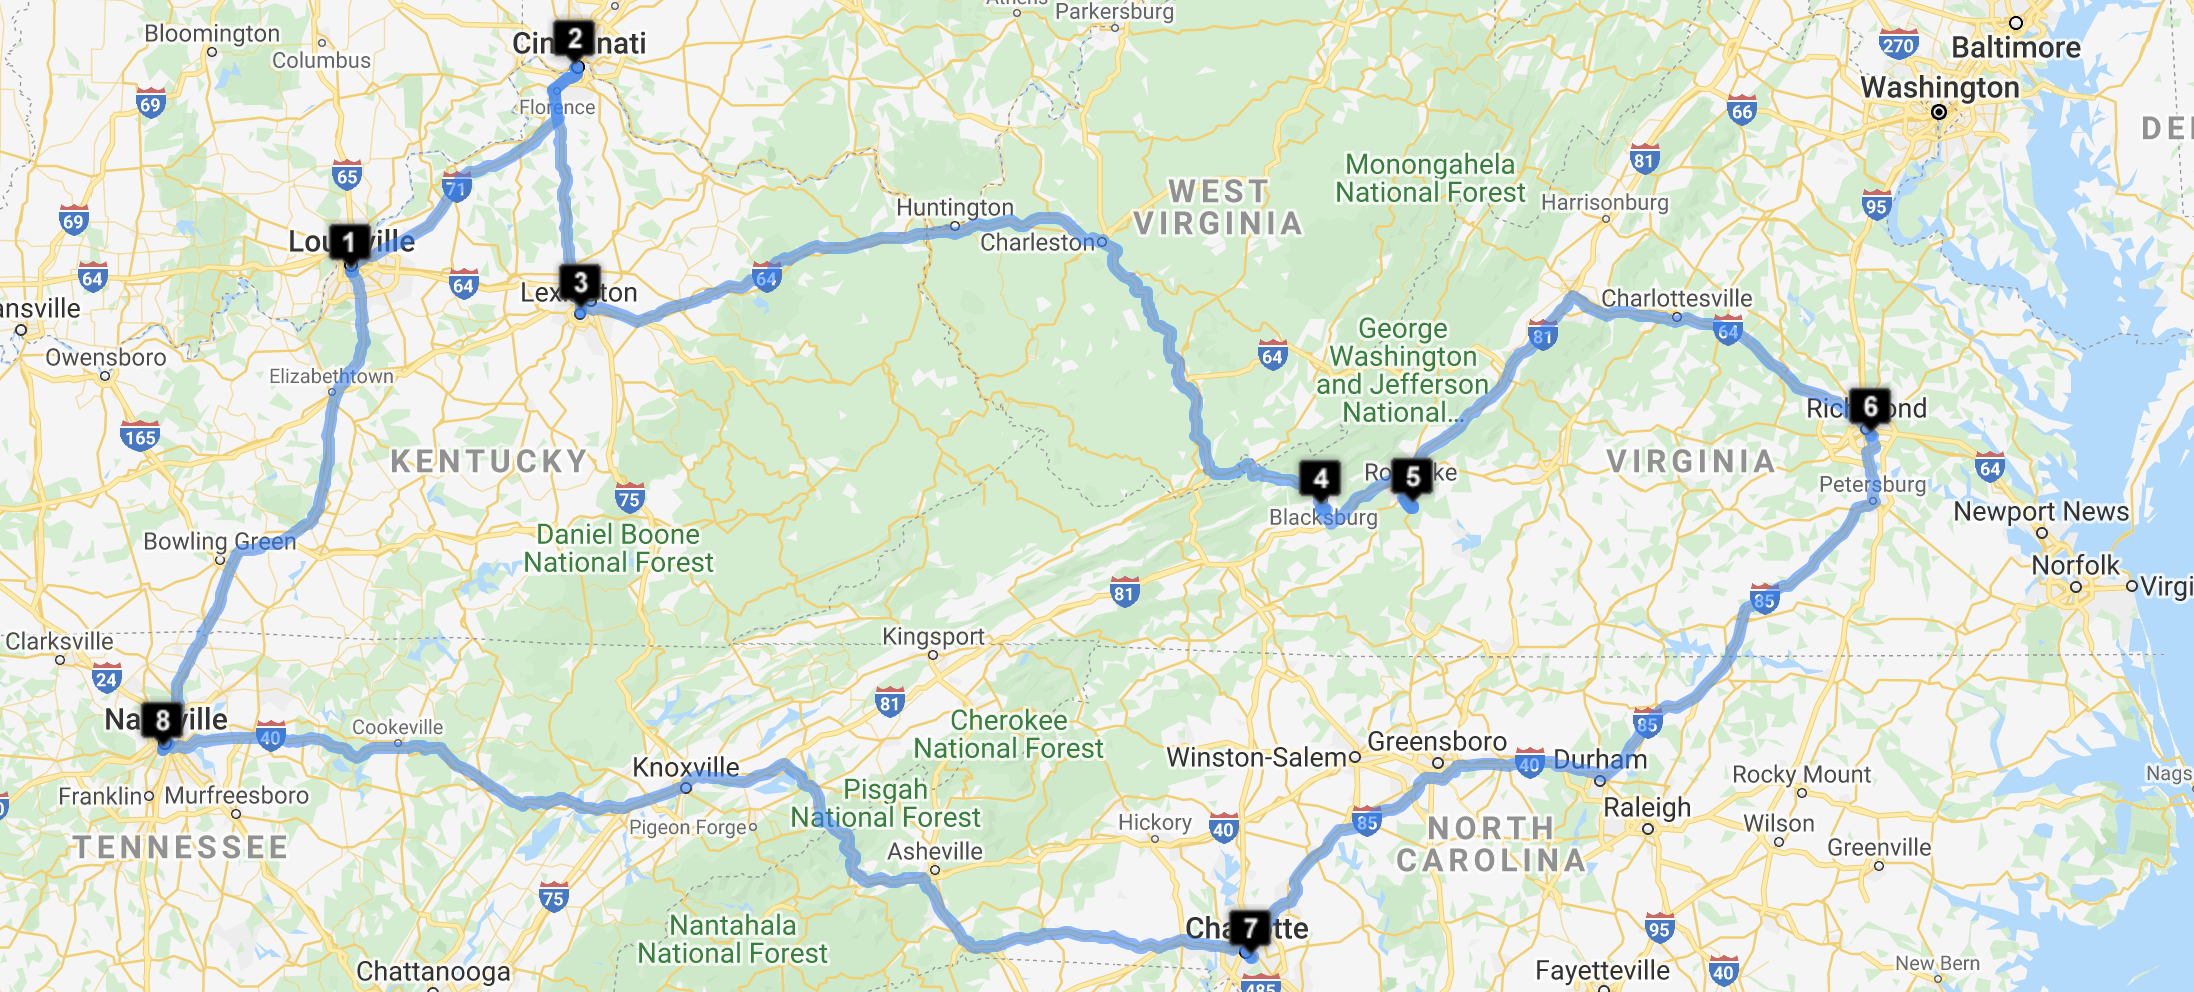
\includegraphics[scale = 0.5]{optimization/figures/figures-static/tsp-optimal-route}
\caption{Optimal tour through 8 cities.  Generated by \href{https://www.gebweb.net/optimap/}{Gebweb - Optimap}.  See it also on \href{https://www.google.com/maps/dir/(38.2222341,+-85.75750389999999)/(39.0972041,+-84.52636389999999)/(38.0493956,+-84.4940986)/(37.1967465,+-80.4296817)/(37.2049884,+-79.9237747)/(37.5110489,+-77.40769019999999)/(35.2019605,+-80.81365720000001)/(36.1303318,+-86.78998039999999)/(38.2222341,+-85.75750389999999)/@36.8110947,-84.2113181,7.02z/data=!4m37!4m36!1m3!2m2!1d-85.7575039!2d38.2222341!1m3!2m2!1d-84.5263639!2d39.0972041!1m3!2m2!1d-84.4940986!2d38.0493956!1m3!2m2!1d-80.4296817!2d37.1967465!1m3!2m2!1d-79.9237747!2d37.2049884!1m3!2m2!1d-77.4076902!2d37.5110489!1m3!2m2!1d-80.8136572!2d35.2019605!1m3!2m2!1d-86.7899804!2d36.1303318!1m3!2m2!1d-85.7575039!2d38.2222341}{Google Maps!}.}
\end{figure}
Aside from actual vehicle routing, the TSP has many applications.  For example, here are some applications related to Industrial Engineering:

\begin{enumerate}
    \item \textbf{Drilling Operations in PCB Manufacturing}: In the production of printed circuit boards (PCBs), there's a need to drill holes at various locations. The TSP can be used to determine the most efficient sequence to drill these holes, minimizing the movement of the drilling head and thereby reducing wear and tear on the machinery and saving time.
    
    \item \textbf{Laser Cutting}: Similar to the PCB example, in industries where laser cutting of materials is required, the TSP can help in determining the optimal path for the laser cutter to follow. This ensures that the material is cut in the shortest time, with minimal movement of the cutting apparatus.
    
    \item \textbf{Robotic Assembly Lines}: In automated assembly lines, robots are often tasked with picking up parts from various locations and assembling them. The TSP can be used to determine the most efficient route for the robot to take, ensuring that products are assembled in the shortest time possible.
    
    \item \textbf{Machine Sequencing}: In factories where multiple machines are used to perform different operations on a workpiece, the TSP can help determine the best sequence of machines to minimize the total processing time and movement of the workpiece.
    
    \item \textbf{Facility Layout}: When designing the layout of a new manufacturing facility or reorganizing an existing one, the TSP can be employed to determine the optimal placement of machinery and workstations. This ensures that materials and products move through the facility in the most efficient manner, reducing transportation costs and times.
    
    \item \textbf{Tool Switching in CNC Machines}: Computer Numerical Control (CNC) machines often have a set of tools that can be switched out depending on the operation. Determining the best order to use these tools to minimize the number of switches (and thus the downtime) can be framed as a TSP.
    
    \item \textbf{Welding Operations}: In industries where welding is a primary operation, determining the sequence of weld joints can be crucial to minimize the movement of the welding torch and ensure efficient utilization of resources. The TSP can be applied to find the optimal sequence.
    
    \item \textbf{Inventory Management}: In large warehouses, picking operations can be optimized using the TSP. When a list of items needs to be picked from various locations in the warehouse, the TSP can help determine the shortest route for the pickers, reducing the time taken to fulfill orders.
\end{enumerate}



\subsection*{Problem statement}
We consider a directed graph, graph $G = (N,A)$ of nodes $N$ and arcs $A$.   Arcs are directed edges.  Hence the arc $(i,j)$ is the directed path $i \to j$.

A \emph{tour}, or Hamiltonian cycle %(see \refincludefigurestatic{wiki/File/William_Rowan_Hamilton_painting.jpg}), 
is a cycle that visits all the nodes in $N$ exactly once and returns back to the starting node. 


Given costs $c_{ij}$ for each arc $(i,j) \in A$, the goal is to find a minimum cost tour.


\begin{general}{Traveling Salesman Problem}{\nphard}
Given a directed graph $G = (N,A)$ and costs $c_{ij}$ for all $(i,j) \in A$, find a tour of minimum cost.
\end{general}
\begin{center}
%\includegraphics[scale = 0.4]{tsp-solution}\footnotemark
\end{center}
In the figure, the nodes $N$ are the cities and the arcs $A$ are the directed paths $\text{city} i \to \text{city} j$.

\paragraph{Models}
When constructing an integer programming model for TSP, we define variables $x_{ij}$ for all $(i,j) \in A$ as 
$$
x_{ij } = 1 \text{ if the arc $(i,j)$ is used  and   }  x_{ij} = 0 \text{   otherwise.}
$$

We want the model to satisfy the fact that each node should have exactly one incoming arc and one leaving arc.  Furthermore, we want to prevent self loops.  Thus, we need the constraints:

\begin{align}
\label{eq:tsp-part-model}
\sum_{j\in N} x_{ij} &= 1 & \text{ for all } i \in N \ \ \text{ [outgoing arc]}\\
\sum_{i \in N} x_{ij} &= 1 & \text{ for all } j \in N \ \ \text{ [incoming arc]}\\
\label{eq:tsp-part-model3}
x_{ii} &= 0 & \text{ for all } i \in N \ \ \text{ [no self loops]} 
\end{align}

Unfortunately, these constraints are not enough to completely describe the problem.  The issue is that \emph{subtours} may arise.  For instance
\begin{figure}[h]
    \centering
    
    % First Graph: Complete directed graph on 7 nodes
%    \begin{tikzpicture}[shorten >=1pt, auto, node distance=2cm, thick]
%        \tikzstyle{vertex}=[circle, draw, minimum size=17pt, inner sep=0pt]
%        
%        \foreach \name/\angle in {A/0, B/51.428, C/102.857, D/154.286, E/205.714, F/257.143, G/308.571}
%            \node[vertex] (\name) at (\angle:2cm) {$\name$};
%        
%        \foreach \from/\to in {A/B, B/C, C/D, D/E, E/F, F/G, G/A, A/C, B/D, C/E, D/F, E/G, F/A, G/B, A/D, B/E, C/F, D/G, E/A, F/B, G/C, A/E, B/F, C/G, D/A, E/B, F/C, G/D, A/F, B/G, C/A, D/B, E/C, F/D, G/E, A/G, B/A, C/B, D/C, E/D, F/E, G/F}
%            \draw[->] (\from) to[bend right=15] (\to);
%    \end{tikzpicture}
    % Second Graph: One 3-cycle and two 2-cycles
    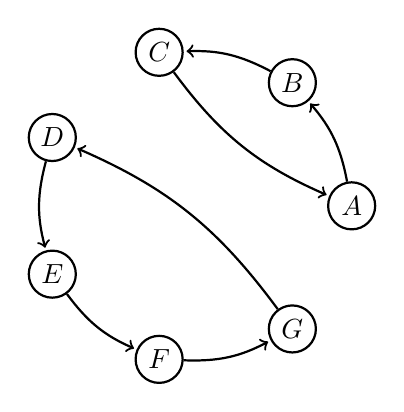
\begin{tikzpicture}[shorten >=1pt, auto, node distance=2cm, thick]
        \tikzstyle{vertex}=[circle, draw, minimum size=17pt, inner sep=0pt]
        
        \foreach \name/\angle in {A/0, B/51.428, C/102.857, D/154.286, E/205.714, F/257.143, G/308.571}
            \node[vertex] (\name) at (\angle:2cm) {$\name$};
        
        \foreach \from/\to in {A/B, B/C, C/A, D/E, E/F, F/G,G/D}
            \draw[->] (\from) to[bend right=15] (\to);
    \end{tikzpicture}
    \hspace{3cm}
    % Third Graph: Hamiltonian tour
    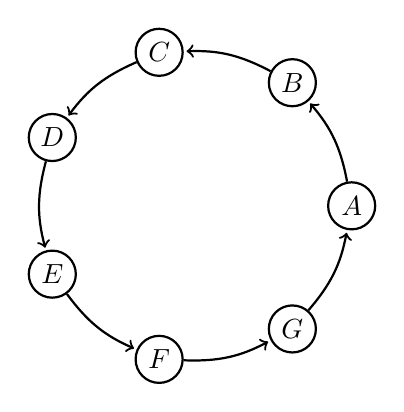
\begin{tikzpicture}[shorten >=1pt, auto, node distance=2cm, thick]
        \tikzstyle{vertex}=[circle, draw, minimum size=17pt, inner sep=0pt]
        
        \foreach \name/\angle in {A/0, B/51.428, C/102.857, D/154.286, E/205.714, F/257.143, G/308.571}
            \node[vertex] (\name) at (\angle:2cm) {$\name$};
        
        \foreach \from/\to in {A/B, B/C, C/D, D/E, E/F, F/G, G/A}
            \draw[->] (\from) to[bend right=15] (\to);
    \end{tikzpicture}
    
    \caption{Left: An assignemnt solution where each node has an incoming arc and an outgoing arc. But in this case, there are 2 subtours.  Right: An assignment that achieves a proper tour.  Note that both of these assignments have the same numbe of arcs!}
\end{figure}

\subsection{Miller Tucker Zemlin (MTZ) Model}
The Miller-Tucker-Zemlin (MTZ) model for the TSP uses varibles to mark the order for which cities are visited.  This model introduce general integer variables to do so, but in the process, creates a formulation that has few inequalities to describe.

Some feature of this model:
\begin{itemize}
\item This model adds variables $u_i \in \Z$ with $1 \leq u_i \leq n$ that decide the order in which nodes are visited.
\item We set $u_1 = 1$ to set a starting place.
\item Crucially, this model relies on the following fact\\
\begin{center}
\emph{
Let  $x$ be a solution to \eqref{eq:tsp-part-model}-\eqref{eq:tsp-part-model3} with $x_{ij} \in \{0,1\}$.  If there exists a subtour in this solution that contains the node $1$, then there also exists a subtour that does not contain the node $1$.}
\end{center}
\end{itemize}

The following model adds constraints
\begin{equation}
\text{ If } x_{ij} = 1, \ \ \text{then} \ \ u_i + 1 \leq u_j.
\end{equation}
This if-then statement can be modeled with a big-M, choosing $M = n$ is a sufficient upper bound.  Thus, it can be written as 
\begin{equation}
\label{mtz-constraint}
u_i + 1 \leq u_j + n(1-x_{ij})
\end{equation}
Setting these constraints to be active enforces the order $u_i < u_j$.    

Consider a subtour now  $2 \to 5 \to 3 \to 2$.  Thus, $x_{25} = x_{53} = x_{32} = 1$.  Then using the constraints from \eqref{mtz-constraint}, we have that 
\begin{equation}
u_2 < u_5 < u_3 < u_2,
\end{equation}
but this is infeasible since we cannot have $u_2 < u_2$.  

As stated above, if there is a subtour containing the node $1$, then there is also a subtour not containing the node $1$.  Thus, we can enforce these constraints to only prevent subtours that don't contain the node $1$.  Thus, the full tour that contains the node $1$ will still be feasible.

This is summarized in the following model:
\begin{general}{Traveling Salesman Problem - MTZ Model}{}
\begin{align}
\min \sum_{i,j \in N} c_{ij} x_{ij}\\
\sum_{j\in N} x_{ij} &= 1 & \text{ for all } i \in N \ \ \text{ [outgoing arc]}\\
\sum_{i \in N} x_{ij} &= 1 & \text{ for all } j \in N \ \ \text{ [incoming arc]}\\
x_{ii} &= 0 & \text{ for all } i \in N \ \ \text{ [no self loops]} \\
u_i + 1 & \leq u_j + n(1-x_{ij})  & \text{ for all } i,j \in N, i,j \neq 1 \ \ \text{[prevents subtours]}\\
u_1 &= 1\\
2 \leq & u_i \leq n & \text{ for all } i \in N, i \neq 1\\
& u_i \in \Z & \text{ for all } i \in N\\
& x_{ij} \in \{0,1\} & \text{ for all } i,j \in N
\end{align}
\end{general}



\begin{example}{MTZ model for TSP with 4 nodes}{}
Consider the distance matrix:
\begin{center}
\begin{tabular}{|c|c|c|c|c|}
\hline
 & 1 & 2 & 3 & 4 \\
\hline
1 & 0 & 1 & 2 & 3 \\
\hline
2 & 1 & 0 & 1 & 2 \\
\hline
3 & 2 & 1 & 0 & 4 \\
\hline
4 & 3 & 2 & 4 & 0 \\
\hline
\end{tabular}
\end{center}

Here is the full MTZ model:
\begin{align*}\min\quad & x_{1,2} + 2 x_{1,3} + 3 x_{1,4} + x_{2,1} + x_{2,3} + 2 x_{2,4} + \\ &2 x_{3,1} + x_{3,2} + 4 x_{3,4} + 3 x_{4,1} + 2 x_{4,2} + 4 x_{4,3}
\end{align*}
\begin{align*}
\text{Subject to} \quad \\
 & x_{1,1} + x_{1,2} + x_{1,3} + x_{1,4} = 1& \text{ outgoing from node 1}\\
  & x_{2,1} + x_{2,2} + x_{2,3} + x_{2,4} = 1& \text{ outgoing from node 2}\\
 & x_{3,1} + x_{3,2} + x_{3,3} + x_{3,4} = 1& \text{ outgoing from node 3}\\
 & x_{4,1} + x_{4,2} + x_{4,3} + x_{4,4} = 1& \text{ outgoing from node 4}\\
 \\
  & x_{1,1} + x_{2,1} + x_{3,1} + x_{4,1} = 1& \text{ incoming to node 1}\\
 & x_{1,2} + x_{2,2} + x_{3,2} + x_{4,2} = 1& \text{ incoming to node 2}\\
 & x_{1,3} + x_{2,3} + x_{3,3} + x_{4,3} = 1& \text{ incoming to node 3}\\ 
 & x_{1,4} + x_{2,4} + x_{3,4} + x_{4,4} = 1& \text{ incoming to node 4}\\
 \\
 & x_{1,1} = 0 & \text{No self loop with node 1}\\
 & x_{2,2} = 0& \text{No self loop with node 2}\\
 & x_{3,3} = 0& \text{No self loop with node 3}\\
 & x_{4,4} = 0& \text{No self loop with node 4}\\
 \\
 & u_{1} = 1 & \text{Start at node 1}\\
  &2  \leq u_{i} \leq 4, \quad\forall i \in \{2,3,4\}\\
 & u_{2} +1 \leq  u_{3} + 4 (1-x_{2,3})\\
 & u_{2} +1 \leq u_{4} + 4 (1-x_{2,4}) \leq 3\\
 & u_{3} +1 \leq u_{2} + 4 (1-x_{3,2}) \leq 3\\
 & u_{3} +1 \leq u_{4} + 4 (1-x_{3,4}) \leq 3\\
 & u_{4} +1 \leq u_{2} + 4 (1-x_{4,2}) \leq 3\\
 & u_{4} +1 \leq u_{3} + 4 (1-x_{4,3}) \leq 3\\
 & x_{i,j} \in \{0,1\} \quad\forall i\in \{1,2,3,4\}, j \in \{1,2,3,4\}\\
 & u_{i} \in \mathbb{Z}, \quad\forall i \in \{1,2,3,4\}\\
\end{align*}
\end{example}


\begin{example}{MTZ model for TSP with 5 nodes}{TSP5node}

\begin{align*}\min\quad & x_{1,2} + 2 x_{1,3} + 3 x_{1,4} + 4 x_{1,5} + x_{2,1} + x_{2,3} + 2 x_{2,4} + 2 x_{2,5} + 2 x_{3,1} + \\&x_{3,2} + 4 x_{3,4} + x_{3,5} + 3 x_{4,1} + 2 x_{4,2} + 4 x_{4,3} + 2 x_{4,5} + \\&4 x_{5,1} + 2 x_{5,2} + x_{5,3} + 2 x_{5,4}
\end{align*}
\begin{align*}
\text{Subject to} \quad  
 & x_{1,1} + x_{1,2} + x_{1,3} + x_{1,4} + x_{1,5} = 1\\
 & x_{2,1} + x_{2,2} + x_{2,3} + x_{2,4} + x_{2,5} = 1\\
 & x_{3,1} + x_{3,2} + x_{3,3} + x_{3,4} + x_{3,5} = 1\\
 & x_{4,1} + x_{4,2} + x_{4,3} + x_{4,4} + x_{4,5} = 1\\
 & x_{5,1} + x_{5,2} + x_{5,3} + x_{5,4} + x_{5,5} = 1\\
 \\
&x_{1,1} + x_{2,1} + x_{3,1} + x_{4,1} + x_{5,1} = 1\\
 & x_{1,2} + x_{2,2} + x_{3,2} + x_{4,2} + x_{5,2} = 1\\
 & x_{1,3} + x_{2,3} + x_{3,3} + x_{4,3} + x_{5,3} = 1\\
 & x_{1,4} + x_{2,4} + x_{3,4} + x_{4,4} + x_{5,4} = 1\\
 & x_{1,5} + x_{2,5} + x_{3,5} + x_{4,5} + x_{5,5} = 1\\
\\
 & x_{1,1} = 0\\
 & x_{2,2} = 0\\
 & x_{3,3} = 0\\
 & x_{4,4} = 0\\
 & x_{5,5} = 0\\
 \\
 & u_{1} = 1\\
 & 2 \leq u_{i} \leq 5 \quad\forall i \in \{1,2,3,4,5\}\\
 & u_{2} +1 \leq u_{3} + 5 (1-x_{2,3})\\
 & u_{2} +1 \leq u_{4} + 5  (1-x_{2,4})\\
  & u_{2} +1 \leq  u_{5} + 5 (1-x_{2,5} )\\
 & u_{3} +1 \leq u_{2} + 5  (1-x_{3,2})\\
 & u_{3} +1 \leq u_{4} + 5  (1-x_{3,4})\\
 & u_{4} +1 \leq u_{2} + 5  (1-x_{4,2})\\
 & u_{4} +1 \leq u_{3} + 5  (1-x_{4,3})\\
 & u_{3} +1 \leq  u_{5} + 5 (1-x_{3,5} )\\
 & u_{4} +1 \leq  u_{5} + 5 (1-x_{4,5})\\
 & u_{5} +1 \leq  u_{2} + 5 (1-x_{5,2} )\\
 & u_{5}+1 \leq  u_{3} + 5 (1-x_{5,3} )\\
 & u_{5} +1 \leq  u_{4} + 5 (1-x_{5,4} )\\
 & x_{i,j} \in \{0,1\} \quad\forall i \in \{1,2,3,4,5\}, j \in \{1,2,3,4,5\}\\
 & u_{i} \in \mathbb{Z}, \quad\forall i \in \{1,2,3,4,5\}
\end{align*}
\end{example}

\paragraph{Pros of this model}
\begin{itemize}
\item Small description
\item Easy to implement
\end{itemize}
\paragraph{Cons of this model}
\begin{itemize}
\item Linear relaxation is not very tight.  Thus, the solver may be slow when given this model.
\end{itemize}

\begin{example}{Subtour elimation constraints via MTZ model}{}
Consider the subtour $2 \to 4 \to 5 \to 2$.   

For this subtour to exist in a solution, we must have

\begin{align*}
x_{2,4} &= 1\\
x_{4,5} &= 1\\
x_{5,2} &= 1.
\end{align*}
Consider the three corresponding inequalities to these variables:

\begin{align*}
u_{2} +1 &\leq  u_{4} + 5 (1-x_{2,4} )\\
u_{4} +1 &\leq  u_{5} + 5 (1-x_{4,5})\\
u_{5} +1 &\leq  u_{2} + 5 (1-x_{5,2} ).
\end{align*}
Since $x_{2,4} = x_{4,5} = x_{5,2} = 1$, these reduce to 
\begin{align*}
u_{2} +1 &\leq  u_{5} \\
u_{4} +1 &\leq  u_{5} \\
u_{5} +1 &\leq  u_{2} .
\end{align*}

Now, lets add these inequalities together.  This produces the inequality

$$
u_2 + u_4 + u_5 + 3 \leq u_2 + u_4 + u_5,
$$
which reduces to
$$
3 \leq 0.
$$
This inequality is invalid, and hence no solution can have the values $x_{2,4} = x_{4,5} = x_{5,2} = 1$.
\end{example}


\begin{example}{Weak Model}{}
Consider again the same tour in the last example, that is, the subtour $2 \to 4 \to 5 \to 2$.  
We are interested to know how strong the inequalties of the problem description are if we allow the variables to be continuous variables.  That is, suppose we relax $x_{ij} \in \{0,1\}$ to be $x_{ij} \in [0,1]$.

Consider the inequalities related to this tour:
\begin{align*}
u_{2} +1 &\leq  u_{4} + 5 (1-x_{2,4} )\\
u_{4} +1 &\leq  u_{5} + 5 (1-x_{4,5})\\
u_{5} +1 &\leq  u_{2} + 5 (1-x_{5,2} ).
\end{align*}

A valid solution to this is 
\begin{align*}
u_2 = 2\\
u_4 = 3\\
u_5 = 4\\
\end{align*}


\begin{align*}
3 &\leq  3 + 5 (1-x_{2,4} )\\
4 &\leq  4 + 5 (1-x_{4,5})\\
5 &\leq  2 + 5 (1-x_{5,2} ).
\end{align*}

\begin{align*}
0&\leq   1-x_{2,4} \\
0&\leq   1-x_{4,5}\\
3 /5&\leq 1-x_{5,2} .
\end{align*}


\begin{align*}
2+1 &\leq  3 + 5 (1-x_{2,4} )\\
3 +1 &\leq  4 + 5 (1-x_{4,5})\\
4 +1 &\leq  2 + 5 (1-x_{5,2} ).
\end{align*}



\end{example}

\begin{comment}

\end{comment}


\subsection{Dantzig-Fulkerson-Johnson (DFJ) Model}
\begin{resource}
\begin{itemize}
\item \href{https://github.com/Gurobi/modeling-examples/tree/master/traveling_salesman}{Gurobi Modeling Example: TSP}
\end{itemize}
\end{resource}
This model does not add new variables.  Instead, it adds constraints that conflict with the subtours.  For instance, consider a subtour
\begin{equation}
2 \to 5 \to 3 \to 2.
\end{equation}
We can prevent this subtour by adding the constraint
\begin{equation}
x_{25} + x_{53} + x_{32}  \leq 2
\end{equation}
meaning that at most 2 of those arcs are allowed to happen at the same time.  In general, for any subtour $S$, we can have the \emph{subtour elimination constraint}
\begin{align}
\sum_{(i,j) \in S} x_{ij} &\leq |S| - 1  & \text{ Subtour Elimination Constraint}.
\end{align}
In the previous example with $S = \{(2,5), (5,3), (3,2)\}$ we have $|S| = 3$, where $|S|$ denotes the size of the set $S$.

This model suggests that we just add all of these subtour elimination constraints.

\begin{general}{Traveling Salesman Problem - DFJ Model}{}
\begin{align}
\label{eq:tsp-DFJ-model}
\min \sum_{i,j \in N} c_{ij} x_{ij}\\
\sum_{j\in N} x_{ij} &= 1 & \text{ for all } i \in N \ \ \text{ [outgoing arc]}\\
\sum_{i \in N} x_{ij} &= 1 & \text{ for all } j \in N \ \ \text{ [incoming arc]}\\
x_{ii} &= 0 & \text{ for all } i \in N \ \ \text{ [no self loops]} \\
\sum_{(i,j) \in S} x_{ij} &\leq |S| -1  & \text{ for all subtours } S \ \ \text{[prevents subtours]}\\
& x_{ij} \in \{0,1\} & \text{ for all } i,j \in N
\end{align}
\end{general}


\begin{example}{DFJ Model for $n=4$ nodes}{}
Consider the distance matrix:
\begin{center}
\begin{tabular}{|c|c|c|c|c|}
\hline
 & 1 & 2 & 3 & 4 \\
\hline
1 & 0 & 1 & 2 & 3 \\
\hline
2 & 1 & 0 & 1 & 2 \\
\hline
3 & 2 & 1 & 0 & 4 \\
\hline
4 & 3 & 2 & 4 & 0 \\
\hline
\end{tabular}
\end{center}

%\begin{center}
%\tikz[nodes={draw, circle}]
%\graph { subgraph K_n [n=4,clockwise,radius=3cm] };
%\end{center}



%\begin{align}\min\quad & x_{1,2} + 2 x_{1,3} + 3 x_{1,4} + x_{2,1} + x_{2,3} + 2 x_{2,4} + 2 x_{3,1} + x_{3,2} + 4 x_{3,4} + 3 x_{4,1} + 2 x_{4,2} + 4 x_{4,3}\\
%\text{Subject to} \quad & x_{1,1} + x_{2,1} + x_{3,1} + x_{4,1} = 1\\
% & x_{1,2} + x_{2,2} + x_{3,2} + x_{4,2} = 1\\
% & x_{1,3} + x_{2,3} + x_{3,3} + x_{4,3} = 1\\
% & x_{1,4} + x_{2,4} + x_{3,4} + x_{4,4} = 1\\
% & x_{1,1} + x_{1,2} + x_{1,3} + x_{1,4} = 1\\
% & x_{2,1} + x_{2,2} + x_{2,3} + x_{2,4} = 1\\
% & x_{3,1} + x_{3,2} + x_{3,3} + x_{3,4} = 1\\
% & x_{4,1} + x_{4,2} + x_{4,3} + x_{4,4} = 1\\
% & x_{1,1} = 0\\
% & x_{2,2} = 0\\
% & x_{3,3} = 0\\
% & x_{4,4} = 0\\
% & x_{i,j} \in \{0,1\} \quad\forall i \in \{1,2,3,4\}, j \in \{1,2,3,4\}\\
%\end{align}


\begin{align*}\min\quad & x_{1,2} + 2 x_{1,3} + 3 x_{1,4} + x_{2,1} + x_{2,3} + 2 x_{2,4} \\& + 2 x_{3,1} + x_{3,2} + 4 x_{3,4} + 3 x_{4,1} + 2 x_{4,2} + 4 x_{4,3}\\
\\
\text{Subject to} \quad \\
 & x_{1,1} + x_{1,2} + x_{1,3} + x_{1,4} = 1& \text{ outgoing from node 1}\\
  & x_{2,1} + x_{2,2} + x_{2,3} + x_{2,4} = 1& \text{ outgoing from node 2}\\
 & x_{3,1} + x_{3,2} + x_{3,3} + x_{3,4} = 1& \text{ outgoing from node 3}\\
 & x_{4,1} + x_{4,2} + x_{4,3} + x_{4,4} = 1& \text{ outgoing from node 4}\\
 \\
  & x_{1,1} + x_{2,1} + x_{3,1} + x_{4,1} = 1& \text{ incoming to node 1}\\
 & x_{1,2} + x_{2,2} + x_{3,2} + x_{4,2} = 1& \text{ incoming to node 2}\\
 & x_{1,3} + x_{2,3} + x_{3,3} + x_{4,3} = 1& \text{ incoming to node 3}\\ 
 & x_{1,4} + x_{2,4} + x_{3,4} + x_{4,4} = 1& \text{ incoming to node 4}\\
 \\
 & x_{1,1} = 0 & \text{No self loop with node 1}\\
 & x_{2,2} = 0& \text{No self loop with node 2}\\
 & x_{3,3} = 0& \text{No self loop with node 3}\\
 & x_{4,4} = 0& \text{No self loop with node 4}\\
 \\
 & x_{1,2} + x_{2,1} \leq 1& S = [(1,2), (2,1)]\\
 & x_{1,3} + x_{3,1} \leq 1& S = [(1,3), (3,1)]\\
 & x_{1,4} + x_{4,1} \leq 1& S = [(1,4), (4,1)]\\
 & x_{2,3} + x_{3,2} \leq 1& S = [(2,3), (3,2)]\\
 & x_{2,4} + x_{4,2} \leq 1& S = [(2,4), (4,2)]\\
 & x_{3,4} + x_{4,3} \leq 1& S = [(3,4), (4,3)]\\
 & x_{2,1} + x_{1,3} + x_{3,2} \leq 2 & S = [(2,1), (1,3), (3,2)]\\
 & x_{1,2} + x_{2,3} + x_{3,1} \leq 2& S = [(1,2), (2,3), (3,1)]\\
 & x_{3,1} + x_{1,4} + x_{4,3} \leq 2& S = [(3,1), (1,4), (4,3))]\\
 & x_{1,3} + x_{3,4} + x_{4,1} \leq 2& S = [(1,3),(3,4), (4,1)]\\
 & x_{2,1} + x_{1,4} + x_{4,2} \leq 2& S = [(2,1), (1,4), (4,2)]\\
 & x_{1,2} + x_{2,4} + x_{4,1} \leq 2& S = [(1,2), (2,4), (4,1)]\\
 & x_{3,2} + x_{2,4} + x_{4,3} \leq 2& S = [(3,2), (2,4), (4,3)]\\
 & x_{2,3} + x_{3,4} + x_{4,2} \leq 2& S = [(2,3), (3,4), (4,2)]\\
 \\
 & x_{i,j} \in \{0,1\} \quad\forall i \in \{1,2,3,4\}, j \in \{1,2,3,4\}\\
\end{align*}
%\includegraphics[scale = 0.5]{CompleteGraph4Nodes}



%\includegraphics[scale = 0.5]{CompleteGraphCycles4-850}\footnotemark
%\footnotetext{\url{http://mathworld.wolfram.com/CompleteGraph.html}}

\end{example}


\begin{example}{}{}

Consider a graph on 5 nodes.

%\begin{center}
%\tikz[nodes={draw, circle}]
%\graph { subgraph K_n [n=5,clockwise,radius=3cm] };
%\end{center}

Here are all the subtours of length at least 3 and also including the full length tours.


Hence, there are many subtours to consider.
\end{example}


\paragraph{Pros of this model}
\begin{itemize}
\item Very tight linear relaxation
\end{itemize}
\paragraph{Cons of this model}
\begin{itemize}
\item Exponentially many subtours $S$ possible, hence this model is too large to write down.
\end{itemize}

\paragraph{Solution: Add subtour elimination constraints as needed}. This is a similar concept as \emph{cutting planes}}.

\subsection{Traveling Salesman Problem - Branching Solution}
We will see in the next section
\begin{enumerate}
\item That the constraint \eqref{eq:tsp-part-model}-\eqref{eq:tsp-part-model3}  always produce integer solutions as solutions to the linear relaxation.
\item A way to use branch and bound (the topic of the next section) in order to avoid subtours.
\end{enumerate}


\subsection{Traveling Salesman Problem Variants}

\subsubsection{Many salespersons (m-TSP)}
\begin{general}{m-Traveling Salesman Problem - DFJ Model}{}
\begin{align}
\label{eq:tsp-DFJ-model}
\min \sum_{i,j \in N} c_{ij} x_{ij}\\
\sum_{j\in N} x_{ij} &= 1 & \text{ for all } i \in N \ \ \text{ [outgoing arc]}\\
\sum_{i \in N} x_{ij} &= 1 & \text{ for all } j \in N \ \ \text{ [incoming arc]}\\
\sum_{j\in N} x_{Dj} &= m & \text{ for all } i \in N \ \ \text{ [outgoing arc]}\\
\sum_{i \in N} x_{iD} &= m & \text{ for all } j \in N \ \ \text{ [incoming arc]}\\
x_{ii} &= 0 & \text{ for all } i \in N\cup\{D\} \ \ \text{ [no self loops]} \\
\sum_{(i,j) \in S} x_{ij} &\leq |S| -1  & \text{ for all subtours } S\subseteq N \ \ \text{[prevents subtours]}\\
& x_{ij} \in \{0,1\} & \text{ for all } i,j \in N\cup\{D\}
\end{align}
\end{general}


When using the MTZ model, you can also easily add in a constraint that restricts any subtour through the deopt to have at most $T$ stops on the tour.  This is done by restricting $u_i \leq T$.  
This could also be done in the DFJ model above, but the algorithm for subtour elimination cuts would need to be modified.

\begin{general}{m-Traveling Salesman Problem - MTZ Model - }{}
\href{https://github.com/open-optimization/open-optimization-or-examples/blob/master/integer-programming/tsp-mtz/m_TSP_with_MTZ_Model.ipynb}{Python Code}
\begin{align}
\min \sum_{i,j \in N} c_{ij} x_{ij}\\
\sum_{j\in N} x_{ij} &= 1 & \text{ for all } i \in N \ \ \text{ [outgoing arc]}\\
\sum_{i \in N} x_{ij} &= 1 & \text{ for all } j \in N \ \ \text{ [incoming arc]}\\
\sum_{j\in N} x_{Dj} &= m & \text{ for all } i \in N \ \ \text{ [outgoing arc]}\\
\sum_{i \in N} x_{iD} &= m & \text{ for all } j \in N \ \ \text{ [incoming arc]}\\
x_{ii} &= 0 & \text{ for all } i \in N\cup\{D\} \ \ \text{ [no self loops]} \\
u_i + 1 & \leq u_j + n(1-x_{ij})  & \text{ for all } i,j \in N, i,j \neq 1 \ \ \text{[prevents subtours]}\\
u_1 &= 1\\
2 \leq & u_i \leq T & \text{ for all } i \in N, i \neq 1\\
& u_i \in \Z & \text{ for all } i \in N\\
& x_{ij} \in \{0,1\} & \text{ for all } i,j \in N\cup\{D\}
\end{align}
\end{general}

\includegraphicstatic{m-tsp_solution}
\href{https://github.com/open-optimization/open-optimization-or-examples/blob/master/integer-programming/tsp-mtz/houses_and_restaurants_assignment.html}{Image html}

\subsubsection{TSP with order variants}
Using the MTZ model, it is easy to provide order variants.  Such as, city 2 must come before city 3
$$
u_2 \leq u_3
$$

or city 2 must come directly before city 3
$$
u_2 + 1 = u_3.
$$

\subsection{Multi vehicle model with capacities}
In this version, we explicitly add extra variable to discuss the routes of each vehicle.   This means that we add another index to the $x$ variable.


Let:
\begin{align*}
c_{ij} & : \text{cost of travel from } i \text{ to } j \\
x_{ijk} & : 
\begin{cases} 
1 & \text{if vehicle } k \text{ travels directly from } i \text{ to } j \\
0 & \text{otherwise}
\end{cases}
\end{align*}

\textbf{Objective:}
\begin{equation}
\min \sum_{i,j} c_{ij} \sum_k x_{ijk}
\end{equation}

\textbf{Subject to:}
\begin{align}
\sum_{i} \sum_{k} x_{ijk} &= 1 & \forall j \neq \text{depot} & \quad \text{(Exactly one vehicle in)} \\
\sum_{j} \sum_{k} x_{ijk} &= 1 & \forall i \neq \text{depot} & \quad \text{(Exactly one vehicle out)} \\
\sum_{i} \sum_{k} x_{ihk} - \sum_{j} \sum_{k} x_{hjk} &= 0 & \forall k, h & \quad \text{(It's the same vehicle)} \\
\sum_{i} q_i \sum_{j} x_{ijk} &\leq Q_k & \forall k & \quad \text{(Capacity constraint)} \\
\sum_{ijk} x_{ijk} &= |S| - 1 & \forall S \subseteq P(N), \ 0 \notin S & \quad \text{(Subtour elimination)} \\
x_{ijk} &\in \{0,1\}
\end{align}


\section{TSP with Time Windows}
Let $G = (V, A)$ be a directed graph where $V$ is the set of nodes (including the depot) and $A$ is the set of arcs. Each arc $(i,j) \in A$ has a cost $c_{ij}$ associated with it which represents the cost of traveling from node $i$ to node $j$. The problem is to find a minimum-cost tour that visits each node within its time window.

Parameters
\begin{itemize}
  \item $n$ - the number of nodes.
  \item $c_{ij}$ - cost of traveling from node $i$ to node $j$.
  \item $[a_i, b_i]$ - time window of node $i$, where $a_i$ and $b_i$ are the earliest and latest time, respectively, that node $i$ can be visited.
  \item $M$ - a large positive number (big-M).
\end{itemize}

Decision Variables
\begin{itemize}
  \item $x_{ij} = 
    \begin{cases} 
      1, & \text{if arc $(i,j)$ is used in the solution} \\
      0, & \text{otherwise}
    \end{cases}$
  \item $t_i$ - time of service beginning at node $i$.
\end{itemize}

Objective Function
\begin{equation}
\text{Minimize } Z = \sum_{i=1}^{n}\sum_{j=1, j \neq i}^{n} c_{ij} x_{ij}
\end{equation}

Constraints:\\
Time Window Constraints
\begin{equation}
a_i \leq t_i \leq b_i \quad \forall i \in V
\end{equation}

Subtour Elimination Constraints
\begin{equation}
t_i + (c_{ij} + s_i - t_j) x_{ij} \leq M(1 - x_{ij}) \quad \forall (i,j) \in A, i \neq j
\end{equation}
where $s_i$ is the service time at node $i$.

Arrival Time Constraints
\begin{equation}
t_j \geq t_i + s_i + c_{ij} - M(1 - x_{ij}) \quad \forall (i,j) \in A, i \neq j
\end{equation}

Flow Conservation Constraints
\begin{equation}
\sum_{j=1, j \neq i}^{n} x_{ij} = 1 \quad \forall i \in V
\end{equation}
\begin{equation}
\sum_{i=1, i \neq j}^{n} x_{ij} = 1 \quad \forall j \in V
\end{equation}

Integer Constraints
\begin{equation}
x_{ij} \in \{0,1\} \quad \forall (i,j) \in A
\end{equation}

\section{Case study - Traveling Salesman Problem Applications for Supply Chain Optimization}

While the traveling salesman problem was built predominantly for applications of a salesman going to distinct locations, a problem that I believe the TSP could be applied to would be supply chain optimization. We could consider the ‘salesman’ in this situation to be a specific product which has to have numerous components appended to the product for the product to be valuable. The iPhone has to go through numerous manufacturing facilities and have numerous components (including antennas, chips and microprocessors) for the phone to be valuable. This problem could be formulated to be a traveling salesman problem. The supply chain manager in this situation would want to ensure that the product gets to each manufacturing facility for the components to be attached to the product. However, we would want to minimize geographic distance traveled. We would furthermore have to consider aspects including whether the manufacturing facility is reliable (would be quantified by some sort of quality score), the amount of product that the manufacturing facility could supply (sometimes special components including materials could be difficult to obtain) and the cost of the manufacturing process (some manufacturing processes would be expensive compared to others). 
There are a couple of interesting features of this supply chain optimization problem which distinguish this against a normal traveling salesman problem. To start, we have to consider numerous factors other than the geographic distance that the product travels. We have to consider factors including cost of process, time to ship (shipping by boat requires time compared to shipping by air) and quality of the manufacturing process. For a phone, electronic robot manufacturing would be reliable compared to human manufacturing, however the cost of human manufacturing in poorer countries would be lower. Phones manufactured in Asia would be cheaper than phones manufactured in the USA, however shipping times would be longer. These features would mathematically have to be built into the model through constraints. Each manufacturing facility could have a specific group of features assigned to the facility. Some electronic manufacturing facilities in the USA could have a quality (Q) = 8, cost (C) = 9 and shipment time (S) = 3. A human manufacturing facility in India could have a quality (Q) = 4, cost (C) = 3 and shipment time (S) = 8. The shipment time scores could be built into the objective function of the model and the quality and cost scores could be built into the constraints. We could have constraints which would decide if a location would be selected if the cost and quality score are there inside a specific target number. I would mathematically incorporate a DFJ model. 
Some other feature that would have to be considered would be if we could have numerous ‘salesmen’ for the supply chain. For highly complex supply chains including cars, there are numerous supply chains for each component of the car. For this supply chain, we could disassemble the car into numerous components (including engines, wheels and electronic components) and build out traveling salesmen algorithms for each of those components. This could be considered a vehicle routing algorithm because of the fact that we are allowed to have numerous supply chains. Furthermore, I could consider the situation if numerous supply chains each require a specific manufacturing facility. We would have to combine the traveling salesman problem and the network flow problem to create a method for managing this. The network flow could figure out if the manufacturing facility has the capacity to create the product. 

\textbf{Data}
I have attached to this paper a Excel data that would be good for building a supply chain optimization model through the TSP. The data includes data of shipment times, expense and throughput rates for manufacturing facilities and which things could be produced by which manufacturing facility. I would build the traveling salesman model to start by figuring out which manufacturing facility is required before the others. I would create the model for the product to go through each manufacturing facility while minimizing cost through shipments and manufacturing cost. I have attached some simple code for the supply chain that includes the cost and capacity constraints, however this model could be extended for other features. We could include that a certain quality score has to be maintained for a facility to be selected. 
The code demonstrates that two subtours could be generated. One subtour is going to be Singapore to Thailand to Mumbai. The other subtour is NY to Chicago to LA. We could then attach a route for LA to Singapore to attach the subtours together. This would lead to a total distance of around 15000 kilometers. I built constraints to this model to ensure that shipment time, cost and quality satisfied constraints.



This supply chain optimization problem differs from a standard TSP in several ways. It involves factors beyond geographic distance, including manufacturing cost, shipping time (e.g., air vs. sea transport), and manufacturing process quality. For instance, electronic robot manufacturing may offer higher reliability but at a greater cost compared to human manufacturing in lower-wage countries. These factors must be incorporated mathematically through constraints. Each manufacturing facility can be assigned specific quality (Q), cost (C), and shipment time (S) scores, which influence the model's objective function and constraints.

\paragraph{Mathematical Model}
The model can incorporate a Decision, Features, and Juxtaposition (DFJ) approach. Constraints determine if a location is selected based on target quality and cost scores. Additional considerations include the possibility of multiple 'salesmen' for complex supply chains, such as in the automotive industry. Each component (e.g., engines, wheels, electronics) can have its TSP algorithm, resembling a vehicle routing problem. Combining TSP and network flow problem techniques can manage these scenarios, with network flow determining manufacturing facility capacity.

\paragraph{Data}

Attached to this paper is Excel data suitable for building a TSP-based supply chain optimization model. The data includes shipment times, expenses, throughput rates, and manufacturing facility-product compatibility. The TSP model starts by identifying the required manufacturing facility and then routes the product through each facility, minimizing costs and considering quality constraints.


\paragraph{Model}


\paragraph{Sets}
\begin{itemize}
    \item $i, j \in$ Facilities: Set of facilities to visit, indexed by $i$ and $j$.
\end{itemize}

\paragraph{Parameters}
\begin{itemize}
    \item $x_{ij} \in \{0, 1\}$: Binary decision variable representing whether to travel from facility $i$ to facility $j$.
    \item $d_{ij}$: Haversine distance between facility $i$ and facility $j$ (calculated based on latitude and longitude).
    \item $Q_{ij}$: Quality score associated with traveling from facility $i$ to facility $j$.
    \item $C_{ij}$: Cost associated with traveling from facility $i$ to facility $j$.
    \item $S_{ij}$: Shipment time associated with traveling from facility $i$ to facility $j$.
\end{itemize}

\paragraph{Objective}
The objective is to minimize the total distance traveled while considering the quality, cost, and shipment time associated with each facility visit:
\begin{equation}
\text{Minimize} \quad \sum_{i \in \text{Facilities}} \sum_{j \in \text{Facilities}, i \neq j} d_{ij} \cdot x_{ij}
\end{equation}

\paragraph{Constraints}
\begin{itemize}
    \item Facility Visit Constraints:
    \begin{equation}
    \sum_{j \in \text{Facilities}, j \neq i} x_{ij} = 1, \quad \forall i \in \text{Facilities}
    \end{equation}
    
    \item Facility Leave Constraints:
    \begin{equation}
    \sum_{i \in \text{Facilities}, i \neq j} x_{ij} = 1, \quad \forall j \in \text{Facilities}
    \end{equation}
    
    \item Quality Score Constraint (Sum of quality scores for selected routes):
    \begin{equation}
    \sum_{i \in \text{Facilities}} \sum_{j \in \text{Facilities}, i \neq j} Q_{ij} \cdot x_{ij} \leq 150
    \end{equation}
    
    \item Cost Constraint (Sum of costs for selected routes):
    \begin{equation}
    \sum_{i \in \text{Facilities}} \sum_{j \in \text{Facilities}, i \neq j} C_{ij} \cdot x_{ij} \leq 250
    \end{equation}
    
    \item Shipment Time Constraint (Sum of shipment times for selected routes):
    \begin{equation}
    \sum_{i \in \text{Facilities}} \sum_{j \in \text{Facilities}, i \neq j} S_{ij} \cdot x_{ij} \leq 100
    \end{equation}
\end{itemize}

\paragraph{Solution}
The Gurobi optimizer is used to solve the TSP model. The optimal solution provides the sequence of facility visits that minimizes the total distance traveled, while meeting quality, cost, and shipment time constraints.



\paragraph{Code}

A simple code sample for the supply chain, incorporating cost and capacity constraints, is provided. This code can be extended to include other features, such as maintaining a specific quality score for facility selection. The code generates two subtours: Singapore to Thailand to Mumbai and NY to Chicago to LA. To connect these subtours, an additional route from LA to Singapore is added, resulting in a total distance of approximately 15,000 kilometers. Constraints ensure that shipment time, cost, and quality meet specified criteria.



\paragraph{Enhancements}

To improve this implementation, the TSP should account for international travel by increasing shipment time constraints.



\section{Vehicle Routing Problem (VRP)}
\todoSection{10\% complete.\\
Add discussion and examples of solving VRP using Google OR tools.
\url{https://www.youtube.com/watch?v=AJ6LeiMe_PQ&t=757s&ab_channel=MixedIntegerProgramming}\\
Add description and link to code for Clark-Wright Algorithm\\
Discuss that there are many many variations of this problem and it is somewhat endless to work on.
}

The VRP is a generlization of the TSP and comes in many many forms.  The major difference is now we may consider multiple vehicles visiting the around cities.
Obvious examples are creating bus schedules and mail delivery routes.  

Variations of this problem include
\begin{itemize}
\item Time windows (for when a city needs to be visited)
\item Prize collecting (possibly not all cities need to be visited, but you gain a prize for visiting each city)
\item Multi-depot vehicle routing problem (fueling or drop off stations)
\item Vehicle rescheduling problem (When delays have been encountered, how do you adjust the routes)
\item Inhomogeneous vehicles (vehicles have different abilities (speed, distance, capacity, etc.).
\end{itemize}

To read about the many variants, see:
\href{https://doi-org.ezproxy.lib.vt.edu/10.1137/1.9781611973594}{
Vehicle Routing: Problems, Methods, and Applications, Second Edition. 
Editor(s): Paolo Toth and Daniele Vigo.  MOS-SIAM Series on Optimization.}


For one example of a VRP model, see \href{https://github.com/Gurobi/modeling-examples/tree/master/technician_routing_scheduling}{GUROBI Modeling Examples - technician routing scheduling}.






\subsection{The Clarke-Wright Saving Algorithm for VRP}
\textbf{[[Under Construction]]}

The Vehicle Routing Problem (VRP) is a classic combinatorial optimization problem that aims to serve a number of customers with a fleet of vehicles in the most cost-effective way. The Clarke-Wright Saving Algorithm is a heuristic approach to solving the VRP. 

\subsection{Concept}

Given a depot and a set of customers, the idea is to evaluate the `savings' that can be achieved by merging two routes into one, instead of serving each customer by a separate route starting and ending at the depot.

\subsection{Saving Calculation}

The saving \(s_{ij}\) of merging the route of customer \(i\) and customer \(j\) is given by:

\begin{equation}
s_{ij} = c(0, i) + c(0, j) - c(i, j)
\end{equation}

Where:
\begin{itemize}
    \item \(c(x, y)\) represents the cost (or distance) between node \(x\) and node \(y\).
    \item \(0\) is the depot.
\end{itemize}

\subsection{Algorithm Steps}

\begin{enumerate}
    \item For each pair of customers \(i\) and \(j\), calculate the saving \(s_{ij}\) and list all the savings in descending order.
    \item Initialize a route for each customer starting and ending at the depot.
    \item Iterate through the savings list. For the largest saving \(s_{ij}\):
    \begin{itemize}
        \item If customers \(i\) and \(j\) can be merged without exceeding vehicle capacity and without violating any route constraints, merge their routes.
        \item Remove individual routes of \(i\) and \(j\).
    \end{itemize}
    \item Repeat step 3 until there are no more feasible merges.
\end{enumerate}

\subsection{Advantages and Limitations}

While the Clarke-Wright Saving Algorithm is computationally efficient and can provide good solutions for the VRP, it is not guaranteed to find the optimal solution. It works best as a starting solution, which can be further improved using other optimization techniques.



\begin{quote}
Borrowed from \url{https://www.researchgate.net/publication/285833854_Chapter_4_Heuristics_for_the_Vehicle_Routing_Problem} \\

The Clarke and Wright Savings Heuristic
The Clarke and Wright heuristic [12] initially constructs back and forth routes $(0, i, 0)$ for $(i=1, \ldots, n)$ and gradually merges them by applying a saving criterion. More specifically, merging the two routes $(0, \ldots, i, 0)$ and $(0, j, \ldots, 0)$ into a single route $(0, \ldots, i, j, \ldots, 0)$ generates a saving $s_{i j}=c_{i 0}+c_{0 j}-c_{i j}$. Since the savings remain the same throughout the algorithm, they can be computed a priori. In the so-called parallel version of the algorithm which appears to be the best (see Laporte and Semet [46]), the feasible route merger yielding the largest saving is implemented at each iteration, until no more merger is feasible. This simple algorithm possesses the advantages of being intuitive, easy to implement, and fast. It is often used to generate an initial solution in more sophisticated algorithms. Several enhancements and acceleration procedures have been proposed for this algorithm (see, e.g., Nelson et al. [59] and Paessens [62]), but given the speed of today's computers and the robustness of the latest metaheuristics, these no longer seem justified.

[12] G. CLARKE AND J. W. WRIGHT, Scheduling of vehicles from a central depot to a number of delivery points, Operations Research, 12 (1964), pp. 568-581.
\end{quote}



%\section{Steiner Tree Problem}
%% GUROBI Vodafone talk
%
%
%Model 1
%\begin{align*}
%\min \ \ \ & \sum_{(u,v) \in E} w_{uv} x_{uv}\\
%\text{ such that }  \ \ \ \\
%x_t & = 1 & \forall t \in T \\
%2x_{uv} - x_u - x_v &\leq 0 &   \forall (u,v) \in E\\
%x_v - \sum_{(u,v) \in E} x_{uv} \leq 0 \forall v \in V\\
%\sum_{(u,v) \in \delta(S)} x_{uv} \geq x_w \forall S \subseteq V, \forall w \in S\\
%\end{align*}
%
%Model 2
%\begin{align*}
%\min &\sum_{(u,v) \in E} w_{uv} x_{uv}\\
%x_t &= 1 &\forall t \in T\\
%2x_{uv} - x_u - x_v &\leq 0 & \forall (u,v) \in E\\
%x_v - \sum_{(u,v) \in E} x_{uv} &\leq 0 &\forall v \in V\\
%x_{uv} + x_{vu} &\leq 1\\
%\sum_{v \in V} x_v - \sum_{(u,v) \in E} x_{uv} &=1&\\
%n x_{uv} + l_v - l_u &\geq 1 - n(1-x_{vu}) &\forall (u,v) \in E\\
%n x_{vu} + l_u - l_v &\geq 1 - n(1-x_{uv}) &\forall (u,v) \in E
%\end{align*}
%
%
%
%
%

\section{Tools to solve VRP}


 There are several tools and software packages available to solve VRPs, ranging from commercial software to open-source libraries. Here are some recommended tools:

\begin{enumerate}
    \item \textbf{Commercial Software}:
    \begin{itemize}
        \item \textbf{Lingo}: A mathematical optimization tool that can be used to model and solve VRPs.
        \item \textbf{IBM ILOG CPLEX Optimization Studio}: Offers powerful optimization modeling capabilities and can solve large-scale VRPs.
        \item \textbf{Gurobi Optimizer}: Another commercial optimization solver that's known for its speed and efficiency.
    \end{itemize}
    
    \item \textbf{Open-Source Solvers}:
    \begin{itemize}
        \item \textbf{OR-Tools}: Developed by Google, OR-Tools is a set of optimization tools that includes solvers for the VRP. It's one of the most popular open-source tools for solving VRPs.
        \item \textbf{JSprit}: A Java-based, open-source toolkit for solving rich VRPs. It's lightweight and can handle various constraints and objectives.
        \item \textbf{VROOM}: A vehicle routing optimization library that focuses on real-world applications with fast execution times.
    \end{itemize}
    
    \item \textbf{Frameworks and Libraries}:
    \begin{itemize}
        \item \textbf{OptaPlanner}: An open-source constraint solver in Java that can tackle VRPs among other planning problems.
        \item \textbf{AequilibraE}: A Python library and QGIS plugin for transportation modeling, including tools for solving VRPs.
    \end{itemize}
    
    \item \textbf{Simulation-Based}:
    \begin{itemize}
        \item \textbf{AnyLogic}: A simulation modeling tool that can be used to model and solve complex VRPs using agent-based, discrete event, and system dynamics simulation methodologies.
    \end{itemize}
    
    \item \textbf{Online Platforms}:
    \begin{itemize}
        \item \textbf{Routific}: A cloud-based route optimization solution that can handle various real-world constraints.
        \item \textbf{OptimoRoute}: An online platform for route planning and optimization suitable for small to medium-sized delivery operations.
    \end{itemize}
    
    \item \textbf{Heuristic and Metaheuristic Approaches}:
    \begin{itemize}
        \item Many researchers and practitioners use heuristic and metaheuristic algorithms like Genetic Algorithms, Simulated Annealing, Tabu Search, and Ant Colony Optimization to solve VRPs. There are various libraries and toolkits in languages like Python, Java, and C++ that can be used to implement these algorithms.
    \end{itemize}
\end{enumerate}

When choosing a tool, consider the following factors:
\begin{itemize}
    \item \textbf{Problem Size}: Some tools are better suited for large-scale problems, while others are designed for smaller instances.
    \item \textbf{Complexity}: If your VRP has many constraints or special requirements, you'll need a more flexible and powerful tool.
    \item \textbf{Budget}: Commercial software can be expensive, but they often come with support and advanced features. Open-source tools are free but might require more time to set up and customize.
    \item \textbf{Programming Skills}: Some tools require programming knowledge, while others offer a graphical interface.
\end{itemize}

Remember that the VRP is NP-hard, which means that as the problem size grows, the time required to find an optimal solution can increase exponentially. In many cases, especially for large problems, heuristic or metaheuristic approaches are used to find good (but not necessarily optimal) solutions in a reasonable amount of time.



\section{Literature and other notes}


\begin{itemize}
\item Gilmore-Gomory Cutting Stock~\cite{Gilmore-Gomory}
\item \href{http://www.optimization-online.org/DB_HTML/2018/06/6648.html}{A Column Generation Algorithm for Vehicle Scheduling and Routing Problems}
\item \href{http://www.optimization-online.org/DB_HTML/2018/06/6670.html}{The Integrated Last-Mile Transportation Problem}
\item \url{http://www.optimization-online.org/DB_FILE/2017/11/6331.pdf}{A BRANCH-AND-PRICE ALGORITHM FOR CAPACITATED
HYPERGRAPH VERTEX SEPARATION}
\end{itemize}




%\begin{resource}
%See~\cite{Abdelmaguid2018} for a list of 11 models for the minimum spanning tree and a comparison using CPLEX.
%\end{resource}
\subsection{TSP In Excel}



%\end{document}
%%% Local Variables:
%%% mode: latex
%%% TeX-master: "../open-optimization/open-optimization"
%%% End:

\subsection{Resources}
TSP
\begin{resource}
See \href{http://www.math.uwaterloo.ca/tsp/index.html}{math.waterloo.ca} for excellent material on the TSP.\\
See also this chapter \href{https://www.math.uwaterloo.ca/~bico/papers/comp_chapter1.pdf}{A Practical Guide to Discrete
Optimization}.

Also, watch this excellent talk by Bill Cook "Postcards from the Edge of Possibility":
\href{https://m.youtube.com/watch?v=5VjphFYQKj8}{Youtube!}

\href{https://www.youtube.com/watch?v=UQYJvSjXE6I}{TSP with excel solver}

Google maps data:
\href{https://www.geeksforgeeks.org/python-calculate-distance-duration-two-places-using-google-distance-matrix-api/}{Blog - Python | Calculate distance and duration between two places using google distance matrix API}
\end{resource}
\begin{resource}
\url{https://www.informs.org/Impact/O.R.-Analytics-Success-Stories/Optimized-school-bus-routing-helps-school-districts-design-better-policies}

\url{https://pubsonline.informs.org/doi/abs/10.1287/inte.2019.1015}

\url{https://www.informs.org/Resource-Center/Video-Library/Edelman-Competition-Videos/2019-Edelman-Competition-Videos/2019-Edelman-Finalist-Boston-Public-Schools}


\url{https://www.youtube.com/watch?v=LFeeaNP_rbY}

\href{https://www.youtube.com/watch?v=BZA_UaX8rs8&t=23s&ab_channel=MERSCognitiveRobotics}{Fantastic talk - Very thorough}

\url{https://www.opendoorlogistics.com/tutorials/tutorial-v-vehicle-routing-scheduling/}
\end{resource}

\begin{resource}
Cutting stock with multiple widths:

Gurobi has as excellent demonstration application to look at:
\href{https://demos.gurobi.com/cutstock/}{Gurobi - Cutting Stock Demo}
\href{https://www.gurobi.com/cutting-stock-problem-with-multiple-master-rolls/}{Gurobi - Multiple Master Rolls}
\end{resource}
